%\title{LaTeX Portrait Poster Template}
%%%%%%%%%%%%%%%%%%%%%%%%%%%%%%%%%%%%%%%%%
% a0poster Portrait Poster
% LaTeX Template
% Version 1.0 (22/06/13)
%
% The a0poster class was created by:
% Gerlinde Kettl and Matthias Weiser (tex@kettl.de)
% 
% Adapter by Jens Buysse for Hogeschool Gent
% This template has been downloaded from:
% http://www.LaTeXTemplates.com
%
% License:
% CC BY-NC-SA 3.0 (http://creativecommons.org/licenses/by-nc-sa/3.0/)
%
%%%%%%%%%%%%%%%%%%%%%%%%%%%%%%%%%%%%%%%%%

%----------------------------------------------------------------------------------------
%	PACKAGES AND OTHER DOCUMENT CONFIGURATIONS
%----------------------------------------------------------------------------------------

\documentclass[a0,portrait]{a0poster}

\usepackage{multicol} % This is so we can have multiple columns of text side-by-side
\columnsep=100pt % This is the amount of white space between the columns in the poster
\columnseprule=3pt % This is the thickness of the black line between the columns in the poster

\usepackage[svgnames]{xcolor} % Specify colors by their 'svgnames', for a full list of all colors available see here: http://www.latextemplates.com/svgnames-colors

\usepackage{times} % Use the times font
%\usepackage{palatino} % Uncomment to use the Palatino font

\usepackage{graphicx} % Required for including images
\graphicspath{{figures/}} % Location of the graphics files
\usepackage{booktabs} % Top and bottom rules for table
\usepackage[font=small,labelfont=bf]{caption} % Required for specifying captions to tables and figures
\usepackage{amsfonts, amsmath, amsthm, amssymb} % For math fonts, symbols and environments
\usepackage{wrapfig} % Allows wrapping text around tables and figures
\usepackage[export]{adjustbox}
\usepackage{subfigure}

\begin{document}

%----------------------------------------------------------------------------------------
%	POSTER HEADER 
%----------------------------------------------------------------------------------------

% The header is divided into two boxes:
% The first is 75% wide and houses the title, subtitle, names, university/organization and contact information
% The second is 25% wide and houses a logo for your university/organization or a photo of you
% The widths of these boxes can be easily edited to accommodate your content as you see fit

\begin{minipage}[t]{0.75\linewidth}
\VeryHuge \color{HoGentAccent1} \textbf{Classificatie van afbeeldingen met geautomatiseerde machine learning platformen} \color{Black}\\[2.4cm] % Title
%\Huge\textit{Ondertitel (eventueel)}\\[2.4cm] % Subtitle
\Huge \textbf{Decorte Robbe, dr. Helsens Kenny, ir. Decorte Johan}\\[0.5cm] % Author(s)
\huge Hogeschool Gent, Valentin Vaerwyckweg 1, 9000 Gent\\[0.4cm] % University/organization
\Large \texttt{robbe.decorte@student.hogent.be} \\
\end{minipage}
%
\begin{minipage}[t]{0.25\linewidth}

\includegraphics[width=13cm,right]{figures/HOGENT_Logo_Pos_rgb.png} 

\end{minipage}

\vspace{1cm} % A bit of extra whitespace between the header and poster content

%----------------------------------------------------------------------------------------

\begin{multicols}{2} % This is how many columns your poster will be broken into, a portrait poster is generally split into 2 columns

%----------------------------------------------------------------------------------------
%	ABSTRACT
%----------------------------------------------------------------------------------------

\color{HoGentAccent1} % Navy color for the abstract

\begin{abstract}
Deze technologie tracht \textit{machine learning} toegankelijker te maken door een manier te bieden om vaak voorkomende problemen te automatiseren. Dit werd onderzocht door met AutoKeras en Google Cloud AutoML elk een prototype op te zetten dat voor een simpel maar realistisch classificatieprobleem de categorie van een afbeelding kan voorspellen. Er werden modellen getraind die katten van honden kunnen onderscheiden. Dit document beschrijft een studie naar de achterliggende gebruikte technieken, het verloop en de resultaten van beide prototypes. Er werd gevonden dat de alternatieven elk hun plaats hebben in verschillende fasen van een project. Google Cloud AutoML levert een productie waardig model terwijl AutoKeras kan dienen als hulpmiddel voor een \textit{data scientist} of productie waardig kan zijn mits een extensieve voorbereiding van de data. De evolutie van de platformen zelf betekent enkel goed nieuws voor de toekomst. Mogelijks kan er nog onderzocht worden hoe het opschonen van de data geautomatiseerd kan worden. Dit is een grote stap binnen geautomatiseerde \textit{machine learning} aangezien het een belangrijke factor is om \textit{edge cases} te herkennen.
\end{abstract}
%----------------------------------------------------------------------------------------
%	INTRODUCTION
%----------------------------------------------------------------------------------------

\color{HoGentAccent1} 
\section*{Introductie}
\color{black}
\color{black}

Het informatie tijdperk centraliseert zich momenteel rond data. Een toepassingen dat intensief gebruik maakt van data, is \textit{machine learning}. Mensen die goed overweg kunnen met de data om zo'n model te maken (Machine Learning Engineers / Data Scientists ...)  zijn vaak moeilijk te vinden. Een werkgever die zo'n probleem aan wilt pakken heeft enkele keuzes, AutoML is een mogelijke optie. Alhoewel het interesseveld ontstaan is in de jaren '50, is het nog maar sinds kort een hot topic, met dank aan de grote hoeveelheid rekenkracht in moderne systemen en doorbraken binnen het onderzoeksveld die de toegangsdrempel verlagen.

Geautomatiseerde \textit{machine learning} platformen trachten een oplossing te bieden voor \textit{development} teams zonder een gespecialiseerde \textit{machine learning} expert. Het platform voert alle stappen van het proces uit en uiteindelijk moeten ze het enkel in hun product integreren. Door de technische afhankelijkheid te verlagen kan de technologie sneller / meer gebruikt worden in bestaande projecten.

%----------------------------------------------------------------------------------------
%	GEOLOGY
%----------------------------------------------------------------------------------------

\color{Black} % DarkSlateGray color for the rest of the content
\color{HoGentAccent1} 
\section*{Experimenten}
\color{black}


\begin{center}\vspace{1cm}
    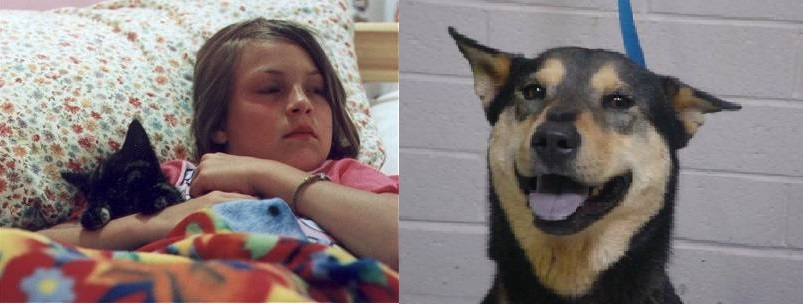
\includegraphics[width=1\linewidth]{./figures/animal.jpg}
    \captionof{figure}{\color{HoGentAccent5}Voorbeelden van afbeeldingen uit de dataset die gebruikt werd om de modellen te trainen.} 
    \label{fig:animals}    
\end{center}

Om de werking van AutoKeras en Google Cloud AutoML te onderzoeken werd voor beide enkele modellen getraind die voorspellen als het object op een afbeelding een kat of een hond is. Figuur \ref{fig:animals} bevat twee afbeeldingen uit de gebruikte dataset. Het experiment blijft realistisch door de afbeeldingen niet te normaliseren (i.e. ook afbeeldingen gebruiken met ruis, zoals het meisje op de eerste foto).

Beide werden beoordeeld op de implementatie van het proces model uit figuur \ref{fig:proces} alsook op extra (niet-) functionele \textit{requirements}.

\begin{center}\vspace{1cm}
    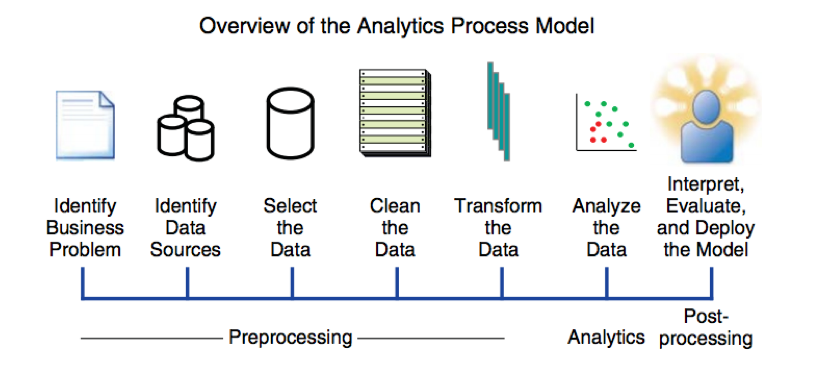
\includegraphics[width=1.0\linewidth]{../bachproef/img/proces-model.png}
    \captionof{figure}{\color{HoGentAccent5}Basisstappen voor een \textit{Data Science} project. Afbeelding via Lemahieu, W., Broucke, S. V. \& Baesens, B. (2018). Principles of Database Management: The Practical Guide to Storing, Managing and Analyzing Big and Small Data. USA, Cambridge University Press.}
    \label{fig:proces}
\end{center}\vspace{1cm}

In het geval van AutoKeras kan er achteraf bekeken worden welke afbeeldingen verkeerd voorspeld werden. Figuur \ref{fig:wrong} bevat negen van die gevallen. Door deze te visualiseren is het mogelijk om een inkijk te krijgen in het model. Zo kom je mogelijks te weten waaraan het model gevoelig is, in dit geval zie je snel dat honden met gespitste oren soms als een kat voorspeld werden.

\begin{center}\vspace{1cm}
    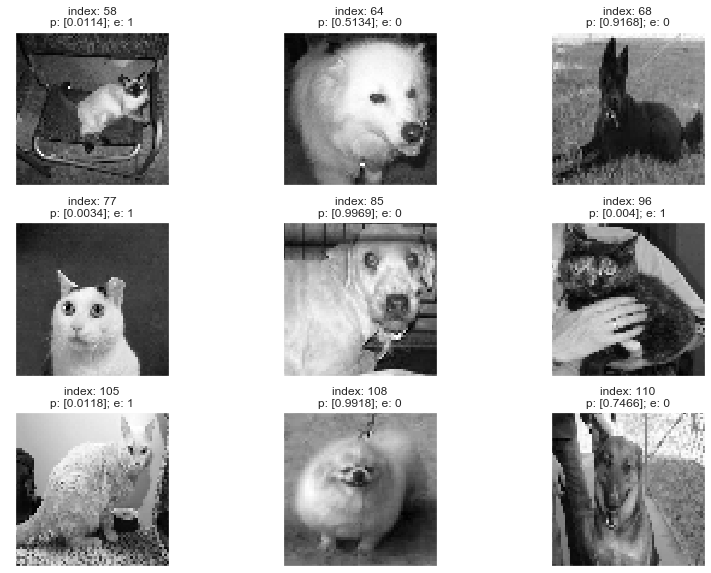
\includegraphics[width=1\linewidth]{./figures/wrong.png}
    \captionof{figure}{\color{HoGentAccent5}Voorbeelden van afbeeldingen die verkeerd geclassificeerd zijn. Bij elke afbeelding staat de zekerheid van de voorspelling (P, [0,0.5[ = hond, ]0.5,1] = kat) en de verwachte klasse (e).} 
    \label{fig:wrong}    
\end{center}

%------------------------------------------------



\color{HoGentAccent1} 
\section*{Conclusies}
\color{black}

Beide systemen komen de verwachtingen na maar moeten op de juiste plaats ingezet worden. Zo is Google Cloud AutoML een volwaardig \textit{drop in replacement} in bestaande applicaties. Het proces kan niet eenvoudiger zijn en de verschillende manieren om het te integreren zorgen ervoor dat het in meeste situaties past. AutoKeras, in zijn huidige staat, is niet verfijnd genoeg om productie waardig te zijn. De extra moeite om de eerste stappen van het procesmodel te verbeteren kan evengoed verwisseld worden met een ML-ingenieur die het volledige proces uitvoert. Die niche kennis blijft noodzakelijk om te slagen. Anderzijds blijkt het wel een goede \textit{tool} te zijn in de gereedschapskist van ML-ingenieurs.

AutoKeras is sterk gericht op de \textit{core} van het probleem en zo blijven stappen vooraf en achteraf onbeantwoord terwijl die bij de werkwijze van Google Cloud AutoML een aanzienlijke rol hebben. Zo kan een model getraind en \textit{deployed} zijn in een vijftal muisklikken, geen vooraf verwerkte afbeeldingen of andere zaken nodig. Dit terwijl AutoKeras pas gebruikt kan worden nadat de afbeeldingen omgezet zijn naar ruwe data, correct geschaald zijn en grijsfilters of andere optimalisaties toegepast worden. Achteraf is het de verantwoordelijkheid van de gebruiker om het model online te krijgen, wachtrij te optimaliseren en een interface te hebben die kan communiceren met het model.

%----------------------------------------------------------------------------------------
%	FORTHCOMING RESEARCH
%----------------------------------------------------------------------------------------
\color{HoGentAccent1} 
\section*{Toekomstig onderzoek}
\color{black}

De toekomst van geautomatiseerde \textit{machine learning} ziet er alvast goed uit. De verbeteringen tussen versies van AutoKeras vallen op en ook steeds meer cloud platformen bieden een gelijkaardige service aan. Er is een echte \textit{push} aan de gang, van de \textit{community} en de bedrijven, om de toepassingen toegankelijker te maken. Verder onderzoek over dit onderwerp zou zich kunnen richten op individuele stappen van het procesmodel, bijvoorbeeld de \textit{data preprocessing}. De automatisatie ervan is niet vanzelfsprekend omdat dit voor elke dataset anders is.


%----------------------------------------------------------------------------------------

\end{multicols}
\end{document}